\nocite{anleitungV601}
\section{Zielsetzung}
\label{sec:Zielsetzung}
Ziel dieses Versuchs ist die Energiedifferenz zwischen dem Grundzustand $E_0$ und des ersten angeregten Zusatnd $E_1$ von Quecksilber mithilfe
eines Elektronenstoßexperiments zu bestimmen. 
\section{Theorie}
\label{sec:Theorie}
Das Franck-Hertz-Experiment zählt zu den Elektronenstoßexperimenten. Hierbei werden \ce{Hg}-Atome mit Elektronen beschossen. Wenn die Elektronen
eine geeignete Energie besitzen, verlieren die Elektronen durch den Stoßprozess Energie. Dieser Energieverlust wird verwendet, um die aufgenommene Energie
der \ce{Hg}-Atome zu bestimmen. Bei unelastischen Stoßprozessen, wird das \ce{Hg}-Atom aus dem Grundzustand $E_0$ auf den Zustand $E_1$ angeregt.
Somit ergibt sich 
\begin{equation}
    E_1 - E_0 =\frac{m_0\cdot v_{\text{vor}^2}}{2} - \frac{m_0\cdot v_{\text{nach}^2}}{2}
    \label{eqn:Energiedifferenz}
\end{equation}
\subsection{Franc k-Hertz-Experiment}
\label{sec:Franck-Hertz-Experiment}
\begin{figure}[H]
  \centering
  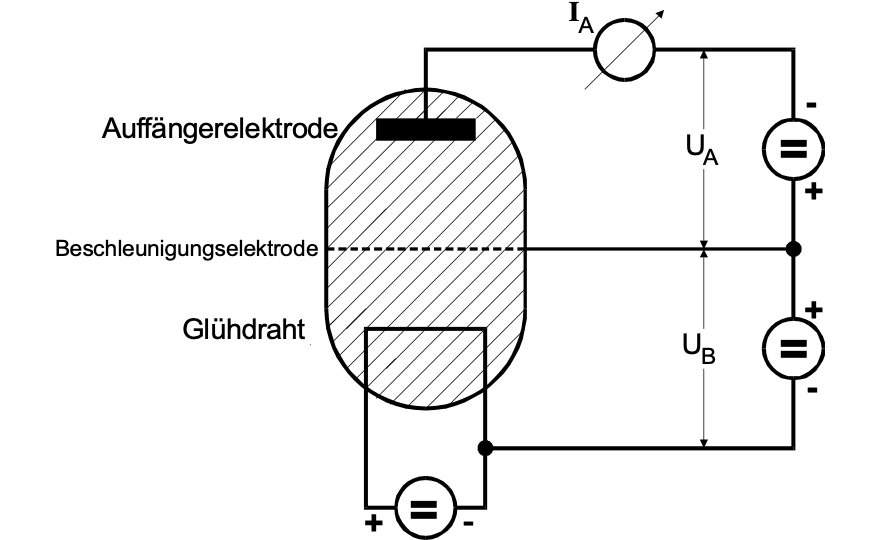
\includegraphics[width=0.6\textwidth]{content/Bilder/schematischerAufbau.png}
  \caption{Schematischer Aufbau des Franck-Hertz-Experiemtns Q\cite{anleitungV601}.}
  \label{fig:schematischerAufbau}
\end{figure}
Eine schematische Darstellung der Franck-Hertz-Apparatur ist in der Abbildung \ref{fig:schematischerAufbau} zu erkennen. Hier befindet sich in einem 
evakuierten Gefäß ein kleiner Tropfen Quecksilber, wovon ein Teil spontan verdampft, bis sich ein Gleichgewichtsdampfdruck $p_{\text{sät}}$ einstellt. 
Dieser ist lediglich von der Umgebungstemperatur $T$ abhängig. Demnach wird mit der Temperatur die Dampfdichte reguliert. 
In dem Glaskolben, befindet sich ein hochschmelzendes Metall, welches durch Gleichstrom bis auf Rotglut erhitzt wird. Eine Elektronenwolke entseteht um den Draht.
Eine netzförmige Elektrode befindet sich gegenüber von dem Glühdraht, an der eine Gleichspannung $U_\text{B}$ angelegt ist. Die Elektronen besitzen nach der Beschleunigung die 
kinetische Energie 
\begin{equation}
    \frac{m_0\cdot v_{\text{vor}}^2}{2}= e_0U_{\text{B}} 
    \label{eqn:E_kin}
\end{equation}
